\chapter{Fundamentação teórica}

Neste capítulo serão definidos vários aspectos do \LaTeX, normas \ac{abnt} e normas institucionais.

\section{\LaTeX}

\LaTeX\ é o nome usual de uma coleção de linguagens e programas para produção, tipografia e diagramação de documentos textuais, para publicação impressa ou digital. Na presente seção, o intuito é apresentar alguns dos detalhes mais relevantes das partes constituintes do \LaTeX.

\subsection{\TeX}

Donald Ervin Knuth\footnote{Célebre cientista da computação e matemático norte"-americano.} criou o \TeX\ porque desejava uma ferramenta adequada para a publicação de seus próprios livros. Knuth também criou o programa \MF\ para criação de fontes para o \TeX. Com o \MF, Knuth criou a família Computer Modern Roman de fontes, a fonte padrão do \TeX. O \TeX\ é uma linguagem e aplicação de tipografia, como sugere o arranjo estilizado das letras de seu próprio nome \cites{Knuth1986a,Knuth1986b,Knuth1986c,Knuth1986d,Knuth1986e}.

A primeira versão do \TeX\ foi lançada em 1978. Sua versão atual, publicada em fevereiro de 2021, é 3.141592653. \TeX\ é software livre, com número de versão que converge para o número \(\pi\), ganhando uma casa decimal a cada atualização. Knuth já manifestou o desejo de congelar o \TeX\ após sua morte, promovendo quaisquer \eng{bugs\/} restantes à \eng{features}.

O \TeX\ é composto por 325 comandos primitivos. Esses comandos são como uma linguagem \eng{assembly\/} para diagramação de textos. A escrita de um documento apenas com esses primitivos não é uma experiência agradável. Porém, uma das grandes vantagens do \TeX\ é sua capacidade de expansão, por meio de macros. O próprio Knuth desenvolveu um formato, chamado de plain \TeX\, onde são definidos cerca de 600 comandos, significativamente mais úteis para autores. O plain \TeX\ é tido como a linguagem básica do \TeX.

É importante distinguir \TeX: a linguagem de tipografia; e \tex: o programa. O programa \tex\ toma um arquivo de texto não"-formatado de codificação \ac{ascii}. É comum o uso da extensão \enquote{.tex}, constituído pelo conteúdo textual e diretivas na linguagem \TeX\ para sua correta diagramação, produzindo, finalmente, um arquivo \ac{dvi}.

É raro o leitor que saiba o quê é um arquivo \ac{dvi}. Há muito o \ac{pdf} se tornou um padrão \lat{de facto\/} para documentos textuais digitais. A própria escrita do TCC, objeto de motivação deste documento, deve ser submetido à biblioteca no formato \ac{pdf}. Há também de se considerar que tanto o \tex\ quanto o \TeX\ foram desenvolvidos tendo a língua inglesa em mente.

Dentre as várias extensões criadas para o \TeX, destaca-se o pdf\TeX. Como o nome sugere, o pdf\TeX é uma extensão do \TeX\ com suporte nativo para criação de \ac{pdf}. A aplicação \pdftex\ é o compilador padrão contemporâneo \cite{Thanh2024}.

\subsection{\LaTeX\ de fato}

Apesar de utilizável, o plain \TeX\ permanece muito primitivo para a grande maioria dos autores. O \LaTeX\ padronizou muitos macros úteis, de alto nível, dando maior usabilidade ao \TeX. O conjunto de macros que constituem o formato \LaTeX\ foi desenvolvido por Leslie Lamport\footnote{Cientista da computação e matemático norte-americano.} no início da década de 1980. A versão atual é o \LaTeXe, atualizada desde sua publicação original, em 1994 \cite{Lamport1994}.

Com o \LaTeX, os autores podem se concentrar apenas no conteúdo de seu texto, deixando todos os aspectos de formatação e diagramação por conta da classe utilizada no \LaTeX. Existem classes ou pacotes \LaTeX\ para virtualmente todas as demandas de escrita, como as normas \ac{abnt}, por exemplo.

Há uma ampla documentação online acerca do \LaTeX, porém a referência autoritativa é tida como o trabalho de Frank Mittelbach, com o \citetitle{Mittelbach2023} \cite{Mittelbach2023}. O formato \LaTeX\ resolve muito das limitações do \TeX, como: suporte mais adequado a textos em outra língua que a inglesa; suporte ao arquivo de entrada \enquote{.tex} codificado em Unicode\footnote{Com \ac{utf8} se tornando o padrão em 2018.}.

O comando comumente usado para processar um arquivo de entrada \enquote{.tex} em um \ac{pdf} (sublimemente formatado) é o \pdflatex. Esse comando consiste apenas em um \eng{alias\/} do \pdftex, com a opção de carregar o formato \LaTeX. Existem mais de 6500 pacotes de estilo expandindo a funcionalidade do \LaTeX. Embora a grande maioria seja altamente especializada e, consequentemente, conhecidos apenas por um nicho da comunidade de usuários, alguns são notórios por sua ubiquidade, sendo considerados \enquote{essenciais} pela maioria dos autores.

\subsection{Distribuições \TeX}

Compiladores, formatos, classes, pacotes, fontes e programas auxiliares. O que se conhece por \LaTeX\ é uma pluralidade de softwares especializados que, operando em conjunto, ajudam autores a produzir documentos de alta qualidade tipográfica. Para auxiliar os autores na tarefa de gerenciar essa enorme coleção de partes, o \LaTeX\ é instalado e mantido através das distribuições \TeX:
\begin{description}
	\item[TeX Live] --- a opção mais comum, com atualizações anuais;
	\item[MacTeX] --- um clone do TeX Live, com algumas configurações especializadas para sistemas macOS;
	\item[MikTeX] --- uma distribuição sólida, mas com alguns potenciais problemas de segurança.
\end{description}
Uma instalação típica do TeX Live fica consome entre 1 e~2~GB de armazenamento. Todas essas distribuições são gratuitas. O \ac{tug}, cujo logo oficial encontra"-se na Figura~\ref{fig:tug}, reúne as instruções básicas de instalação e uso das distribuições \TeX.

\begin{figure}
	\caption{Logo do \ac{tug}.}
	\label{fig:tug}
	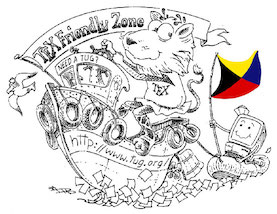
\includegraphics{./figuras/tug}
	\legend{Fonte~---~\cite{tug2024}.}
\end{figure}

Atualmente, muitos autores sequer dão"-se ao trabalho de manter uma instalação local. Plataformas online como o Overleaf expandem a comunidade de autores em \LaTeX\ por sua conveniência.

Um problema notório do Overleaf, que tem se agravado recentemente, é a limitação da capacidade de sua licença gratuita. Como uma empresa, o Overleaf deseja vender o maior número de licenças comerciais possível. Para promover essa meta, tem reduzido muito o tempo máximo de compilação de usuários sem licença. Isso pode ser um impedimento na produção de uma monografia acadêmica, com várias dezenas de páginas.

\subsection{A classe \memoir}

A classe \memoir\ é uma classe flexível para a tipografia de textos de poesia, ficção, não"-ficção e matemática, como livros, relatórios, artigos ou manuscritos. Documentos podem usar tamanhos de fonte de 9~pt, 10~pt, 11~pt, 12~pt, 14~pt ou 17~pt como tamanho normal de fonte. Muitos métodos são oferecidos para criação de formatações particulares. A classe incorpora mais de 30 pacotes populares \cite{memoir2001}.

No \LaTeX\, apenas uma classe pode ser utilizada por documento. A classe \memoir\ é uma boa opção para usar como base de uma classe própria, por expandir (e muito) as estruturas disponibilizadas pelas classes padrão do \LaTeX.

\subsection{Pacotes}

Para autores interessados apenas em escrever suas monografias, sem ter um curso completo de \LaTeX, a principal distinção entre pacotes e classes é que podemos utilizar múltiplos pacotes em um mesmo documento. Os pacotes são utilizados para modificar e expandir o comportamento da classe.

\subsubsection{Babel}

Por exemplo, o pacote \babel\ provê funcionalidades para escrever textos em línguas que não a inglesa, ajustando questões como nomes de seções e hifenização de palavras. É raro que pacotes sejam incompatíveis entre si, ou com alguma classe. É importante se familiarizar com a documentação dos pacotes utilizados.

\section{Normas ABNT}

A simples menção das \enquote{normas \ac{abnt}} já foi suficiente para causar arrepios na espinha dorsal de qualquer acadêmico. Isso ainda era piorado pelo fato de muitos docentes (mesmo com anos de carreira) desconhecerem as normas. Grupos de docentes, inadvertidamente, consolidavam entendimentos errôneos sobre as normas.

As chamadas normas \ac{abnt} são individualmente denominadas por \ac{nbr} e enumeradas sequencialmente. No momento desta escrita, as normas atualizadas\footnote{Pertinentes ao presente esforço.} são:
\begin{itemize}
	\item \citetitle{NBR6023} \cite{NBR6023};
	\item \citetitle{NBR6024} \cite{NBR6024};
	\item \citetitle{NBR6027} \cite{NBR6027};
	\item \citetitle{NBR6028} \cite{NBR6028};
	\item \citetitle{NBR10520} \cite{NBR10520};
	\item \citetitle{NBR14724} \cite{NBR14724};
\end{itemize}

Apesar da má fama, as normas \ac{abnt} são, em sua grande maioria, simples e razoáveis. As exceções são as normas de Citações \cite{NBR10520} e de Referências \cite{NBR6023}, as quais são um pouco mais nebulosas, especialmente a última. Por sorte, existem pacotes com uma implementação \enquote{perfeita} dessas normas, simplificando (e muito) o trabalho dos autores.

\section{Normas da UTFPR}

As normas da UTFPR estão expressas em três documentos institucionais:
\begin{description}
	\item[\citetitle{cogep2021}] --- Dispõe sobre a política de licenciamento das versões finais dos Trabalhos de Conclusão de Curso da Graduação e da Pós"-Graduação \lat{Lato\/} e \lat{Stricto Sensu\/} (dissertações e teses), bem como dos produtos educacionais e tecnológicos a elas vinculados, produzidos no âmbito da UTFPR \cite{cogep2021};
	\item[\citetitle{prograd2021}] --- Estabelece normas e procedimentos operacionais para o depósito de versões finais de Trabalhos de Conclusão de Cursos de Graduação da UTFPR nas Bibliotecas para a disponibilização no Repositório Institucional da UTFPR \cite{prograd2021}.
\end{description}

Ademais, também é considerado o documento institucional específico do curso de Bacharelado em Engenharia Eletrônica da UTFPR campus Campo Mourão:
\begin{description}
	\item[\citetitle{coele2023}] --- Dispõe sobre as Normas Complementares para Trabalho de Conclusão de Curso do Curso de Bacharelado em Engenharia Eletrônica da \ac{utfpr} \cite{coele2023}.
\end{description}
